\documentclass[12pt]{article}
\usepackage[a4paper, margin=1in]{geometry}
\usepackage{setspace}
\usepackage{enumitem}
\usepackage{hyperref}
\usepackage{graphicx}
\usepackage{caption}
\usepackage{float}
\usepackage{listings}
\usepackage{xcolor}
\usepackage{tikz}
\usepackage{multirow}
\usepackage{array}

\lstset{
  basicstyle=\ttfamily\small,
  breaklines=true,
  columns=fullflexible,
  commentstyle=\color{gray},
  keywordstyle=\color{blue},
  stringstyle=\color{red}
}

\title{\textbf{ERP Clone - Educational Institute Management System \\ Comprehensive Project Report}}
\author{
\begin{tabular}{c}
\textbf{K. Saravanarjun} \\ Roll No: 23CS01028 \\[0.5em]
\textbf{M. Shashikanth} \\ Roll No: 23CS01037 \\[0.5em]
\textbf{Vikranth M} \\ Roll No: 23CS02014
\end{tabular}
}
\date{\today}

\begin{document}

\maketitle
\onehalfspacing

\tableofcontents
\newpage

\section*{Abstract}

The ERP Clone project is a comprehensive enterprise resource planning system that integrates Educational Institute Management System (EIMS) functionalities with a banking module within a unified platform. The system is designed to digitize institutional operations through a full-stack architecture composed of a React-based frontend, Express.js backend, and PostgreSQL database.

The EIMS module handles academic administration including student and faculty management, course registration with prerequisite validation, attendance tracking, grade management, fee processing, supplementary examinations, leave request handling, and placement-related activities. The banking module provides complementary financial services such as customer account management, balance inquiry, fund transfers, transaction history, and payment processing.

The system emphasizes role-based access control with three primary user roles: Student, Faculty, and Administrator. Each role has distinct access permissions and workflows designed to mirror real-world academic and administrative processes. The database layer implements comprehensive constraints, triggers, stored procedures, and views to enforce business rules and automate workflows directly at the data level, ensuring data consistency and integrity across all operations.

\newpage

\section{System Architecture Overview}

\subsection{Technology Stack}

\begin{itemize}
    \item \textbf{Frontend:} React.js with Bootstrap CSS framework for responsive user interfaces
    \item \textbf{Backend:} Express.js with Node.js runtime on port 5000
    \item \textbf{Database:} PostgreSQL with comprehensive schema design
    \item \textbf{Authentication:} JWT-based login with bcrypt password hashing and legacy migration support
    \item \textbf{Automation:} Node Cron for scheduled cleanup and data management tasks
\end{itemize}

\subsection{Project Structure}

The project is organized into three distinct modules:

\begin{enumerate}
    \item \textbf{eims-frontend:} React components for student, faculty, and admin dashboards
    \item \textbf{eims-backend:} Express.js API endpoint handling all EIMS operations
    \item \textbf{eims-db:} PostgreSQL schema with 31 tables, views, stored procedures, and triggers
    \item \textbf{bank-frontend:} Separate React application for banking functionalities
    \item \textbf{bank-backend:} Banking API endpoints (separate from EIMS)
    \item \textbf{bank-db:} Banking schema with 4 core tables
\end{enumerate}

\newpage

\section{Database Schema Design}

\subsection{EIMS Database Overview}

The EIMS database consists of 31 interconnected tables organized into functional groups:

\subsubsection{User Management}
\begin{itemize}
    \item \textbf{Users:} Core authentication table storing user credentials and roles (Student, Faculty, Admin)
\end{itemize}

\subsubsection{Academic Structure}
\begin{itemize}
    \item \textbf{Departments:} Institutional departments with head faculty reference
    \item \textbf{Discipline:} Academic programs (B.Tech, M.Tech) with fee and semester information
    \item \textbf{Students:} Student profiles linked to departments and disciplines
    \item \textbf{Faculty:} Faculty profiles with department assignments
    \item \textbf{Faculty\_Advisor:} Mapping of students to faculty advisors for guidance and leave approvals
\end{itemize}

\subsubsection{Course Management}
\begin{itemize}
    \item \textbf{Courses:} Course masters with credits and department linkage
    \item \textbf{Prerequisites:} Course dependency relationships defining course progression
    \item \textbf{Course\_Offerings:} Specific course instances with faculty, semester, and capacity details
    \item \textbf{Course\_Allotted:} Final student enrollments in specific course offerings
    \item \textbf{Course\_Registration:} Temporary workflow table for registration with approval tracking
\end{itemize}

\subsubsection{Academic Performance}
\begin{itemize}
    \item \textbf{Attendance:} Daily attendance records by student and course
    \item \textbf{Grades:} Final grades assigned to students per course offering
    \item \textbf{Results:} Cumulative GPA (CGPA) and total credit computation
    \item \textbf{Backlogs:} Failed courses that require retaking
    \item \textbf{Supplementary\_Exams:} Supplementary examination registrations for failed subjects
\end{itemize}

\subsubsection{Examination Management}
\begin{itemize}
    \item \textbf{Exams:} Examination schedules and details per course offering
    \item \textbf{Exam\_Seating:} Seating allocations for examinations
    \item \textbf{Rooms:} Classroom resources indexed by building and room number
    \item \textbf{Scheduled\_Class:} Class timetables linking courses to rooms and time slots
    \item \textbf{booked\_class:} Additional or alternate class bookings made by faculty
\end{itemize}

\subsubsection{Student Services}
\begin{itemize}
    \item \textbf{Feedback:} Course feedback submitted by students for continuous improvement
    \item \textbf{Leave\_Requests:} Leave applications from students with approval workflow
    \item \textbf{On\_Leave:} Approved leave records linked to requests
    \item \textbf{Fee\_Payment:} Student fee payment transactions and history
    \item \textbf{Balance:} Remaining fee balance per student
    \item \textbf{Fee\_Remission\_Application:} Fee waiver requests with approval status
\end{itemize}

\subsubsection{Placement and Career Services}
\begin{itemize}
    \item \textbf{CDC:} Placement and internship opportunities from companies
    \item \textbf{CDC\_Eligible\_Departments:} Department-wise eligibility criteria for placements
    \item \textbf{CDC\_Applications:} Student applications with multi-stage evaluation (online test, interview, final offer)
\end{itemize}

\subsubsection{Configuration}
\begin{itemize}
    \item \textbf{System\_Config:} Global configuration parameters (registration dates, fee portal status, etc.)
\end{itemize}

\subsection{Banking Database Overview}

The banking schema complements EIMS with transaction-oriented functionality:

\begin{itemize}
    \item \textbf{Customers:} Customer registration with email uniqueness constraint
    \item \textbf{Accounts:} Customer accounts with balance tracking and account type (savings/current)
    \item \textbf{Transactions:} Individual debit and credit entries for accounts
    \item \textbf{Transfers:} Fund transfer records between accounts with validation
\end{itemize}

\newpage

\section{Detailed Role-Based Functionalities}

\subsection{Student Functionalities}

Students have access to comprehensive academic, administrative, and financial services through the EIMS system. The following sections detail each functionality available to students.

\subsubsection{Authentication and Profile Management}

\paragraph{1. Sign Up Process}
\begin{itemize}
    \item \textbf{Endpoint:} \texttt{POST /signup}
    \item \textbf{Parameters:} user\_id, password, role, and profile-specific fields
    \item \textbf{Validation:} 
        \begin{itemize}
            \item Password must contain at least 1 uppercase letter, 1 digit, and 1 special character
            \item User ID must be unique in the system
        \end{itemize}
    \item \textbf{Actions:}
        \begin{itemize}
            \item Creates entry in Users table with hashed password using bcrypt
            \item Creates corresponding entry in Students table with profile information
            \item Associates student with department, discipline, and academic year
            \item Initializes student as current semester 1
        \end{itemize}
    \item \textbf{Return:} Success confirmation or validation error message
\end{itemize}

\paragraph{2. Login}
\begin{itemize}
    \item \textbf{Endpoint:} \texttt{POST /login}
    \item \textbf{Parameters:} user\_id, password
    \item \textbf{Validation:}
        \begin{itemize}
            \item Checks if user exists in Users table
            \item Compares provided password with stored hash using bcrypt
            \item Supports legacy migration by accepting and upgrading plain-text passwords
        \end{itemize}
    \item \textbf{Return:} User role (Student/Faculty/Admin) upon successful authentication, error otherwise
\end{itemize}

\paragraph{3. Profile Retrieval and Update}
\begin{itemize}
    \item \textbf{Endpoints:}
        \begin{itemize}
            \item \texttt{GET /student/profile/:id} - Retrieves complete student profile
            \item \texttt{POST /student/profile} - Updates student profile information
        \end{itemize}
    \item \textbf{Updatable Fields:} student\_name, contact\_no, college\_email, personal\_email, residence\_address, join\_date, semester, department\_id, discipline\_id
    \item \textbf{Return:} Updated profile data or error message
\end{itemize}

\subsubsection{Course Registration and Management}

Course registration is a critical workflow in the EIMS system with multiple stages and validations.

\paragraph{Workflow: Course Registration Process}

\begin{enumerate}
    \item \textbf{View Available Courses} (\texttt{GET /student/registrations/:id})
        \begin{itemize}
            \item Fetches Student\_Registration\_View populated with eligible courses
            \item Displays courses within student's discipline with capacity information
            \item Shows prerequisite satisfaction status
            \item Indicates approval status (selected, approved, or open)
        \end{itemize}
    
    \item \textbf{Select Courses} (\texttt{POST /student/registration})
        \begin{itemize}
            \item Student selects desired courses from available options
            \item System verifies registration window is open via System\_Config check
            \item If window closed, returns 403 error "Registration window closed"
            \item Updates selected flag in Course\_Registration table
            \item Does not trigger approval phase at this stage
        \end{itemize}
    
    \item \textbf{Database Validations (Automated via Triggers)}
        \begin{itemize}
            \item \textbf{Prerequisite Validation:} Trigger \textit{trg\_check\_prerequisites} verifies student has completed all prerequisite courses with passing grade
            \item \textbf{Capacity Check:} Trigger \textit{trg\_course\_capacity} ensures course enrollment does not exceed capacity
            \item \textbf{Duplicate Prevention:} Checks student not already enrolled in same course
        \end{itemize}
    
    \item \textbf{Faculty Approval Phase} (\texttt{GET /faculty/pending/:faculty\_id} and \texttt{POST /faculty/approve})
        \begin{itemize}
            \item Faculty advisor retrieves pending course selections from students
            \item Reviews each student's course selections and prerequisites
            \item Approves or denies individual course registrations
            \item Upon final approval, trigger \textit{trg\_course\_approval} automatically:
                \begin{itemize}
                    \item Moves record from Course\_Registration to Course\_Allotted (final enrollment table)
                    \item Deletes from temporary Course\_Registration table
                    \item Marks course as officially enrolled
                \end{itemize}
        \end{itemize}
\end{enumerate}

\paragraph{Important Constraints:}
\begin{itemize}
    \item Registration window must be open (checked via System\_Config)
    \item All prerequisites must be satisfied with passing grades
    \item Course capacity must not be exceeded
    \item Student cannot register for same course twice
    \item Approval cannot occur without prior selection (database enforced: approved = FALSE OR selected = TRUE)
\end{itemize}

\subsubsection{Academic Performance Tracking}

\paragraph{1. View Current Courses and Grades}
\begin{itemize}
    \item \textbf{Endpoint:} \texttt{GET /student/:id/current-courses}
    \item \textbf{Source:} Student\_Current\_Sem\_Courses\_Grades view
    \item \textbf{Data Returned:} course\_name, credits, grade for current semester courses
    \item \textbf{Purpose:} Students track their current semester academic performance
\end{itemize}

\paragraph{2. View CGPA and Overall Results}
\begin{itemize}
    \item \textbf{Endpoint:} \texttt{GET /student/:id/cgpa}
    \item \textbf{Source:} Results table - populated by system after result declaration
    \item \textbf{Data Returned:} cgpa (0-10 scale), total\_credits accumulated
    \item \textbf{Calculation:} CGPA computed from all semester grades using standard credit-weighted formula
    \item \textbf{Note:} Value becomes available after admin declares results
\end{itemize}

\paragraph{3. View Semester-wise Transcript}
\begin{itemize}
    \item \textbf{Endpoint:} \texttt{GET /student/:id/semester/:sem/transcript}
    \item \textbf{Source:} Student\_All\_Semester\_Grades view
    \item \textbf{Data Returned:} Courses taken in specified semester with grade and credit information
    \item \textbf{Use:} Academic transcript generation and verification
\end{itemize}

\paragraph{4. View Current Semester SGPA}
\begin{itemize}
    \item \textbf{Endpoint:} \texttt{GET /student/:id/current-sgpa}
    \item \textbf{Source:} current\_sem\_sgpa view
    \item \textbf{Data Returned:} Current semester and corresponding SGPA
    \item \textbf{Purpose:} Track performance in current ongoing semester
\end{itemize}

\paragraph{5. View Previous Semester GPAs}
\begin{itemize}
    \item \textbf{Endpoint:} \texttt{GET /student/:id/previous-sgpa}
    \item \textbf{Source:} Student\_Previous\_SGPA view
    \item \textbf{Data Returned:} Complete history of SGPA by semester
    \item \textbf{Purpose:} Analyze academic trends over time
\end{itemize}

\paragraph{6. View Grades by Offering}
\begin{itemize}
    \item \textbf{Endpoint:} \texttt{GET /student/:id/grades}
    \item \textbf{Source:} Grades table with Courses and Course\_Offerings join
    \item \textbf{Data Returned:} grade, course\_name, course\_id, semester, year\_offering, faculty\_id
    \item \textbf{Sorting:} Sorted by year and semester in descending order
\end{itemize}

\subsubsection{Attendance Management}

\paragraph{1. View Attendance Summary}
\begin{itemize}
    \item \textbf{Endpoint:} \texttt{GET /student/:id/attendance}
    \item \textbf{Source:} Student\_Attendance\_Summary view
    \item \textbf{Data Returned:} Course-wise present and absent counts
    \item \textbf{Purpose:} Students monitor their overall attendance across all courses
    \item \textbf{Note:} Aggregated from Attendance table at course offering level
\end{itemize}

\paragraph{2. Faculty Marks Attendance (Faculty Endpoint)}

While faculty mark attendance, students see the results through the above endpoint:
\begin{itemize}
    \item \textbf{Endpoint:} \texttt{POST /faculty/mark-attendance}
    \item \textbf{Parameters:} course\_offering\_id, date, attendance array with student\_id and is\_present flag
    \item \textbf{Execution:} Calls mark\_attendance() stored procedure
    \item \textbf{Database Operation:}
        \begin{itemize}
            \item Inserts entries into Attendance table with student\_id, course\_offering\_id, class\_date, and status
            \item Status values: Present, Absent, or On\_Leave (check constraint enforced)
            \item On\_Leave status automatically applied if student is in On\_leave record for that date
        \end{itemize}
\end{itemize}

\subsubsection{Fee Payment and Financial Management}

\paragraph{1. View Fee Status}
\begin{itemize}
    \item \textbf{Endpoint:} \texttt{GET /student/:id/fee-status}
    \item \textbf{Data Returned:}
        \begin{itemize}
            \item Overall: total\_fee, amount\_paid, net\_payable (remaining balance)
            \item Semester-wise breakdown: fee\_amount, paid\_amount, balance, status for each semester
        \end{itemize}
    \item \textbf{Calculation:}
        \begin{itemize}
            \item Total fees fetched from Discipline table based on student's discipline\_id
            \item Amount paid computed from Fee\_Payment table
            \item Remaining balance fetched from Balance table
        \end{itemize}
    \item \textbf{Status Indicators:}
        \begin{itemize}
            \item \textit{paid:} Full fee paid for that semester
            \item \textit{pending:} Partial or no payment, registration still open
            \item \textit{overdue:} Registration deadline passed without payment
        \end{itemize}
\end{itemize}

\paragraph{2. Initiate Fee Payment}
\begin{itemize}
    \item \textbf{Endpoint:} \texttt{POST /student/:id/pay}
    \item \textbf{Parameters:} semester, amount\_paid
    \item \textbf{Validations:}
        \begin{itemize}
            \item Checks is\_fees\_open flag in System\_Config (admin controlled)
            \item Returns 403 "Fee payment is currently closed by admin" if disabled
        \end{itemize}
    \item \textbf{Return:} Payment URL redirect to payment gateway (currently mocked as localhost:4000)
    \item \textbf{Process:} Contains student\_id, semester, and amount parameters for payment processing
\end{itemize}

\paragraph{3. Record Payment Success}
\begin{itemize}
    \item \textbf{Endpoint:} \texttt{POST /student/payment-success}
    \item \textbf{Parameters:} student\_id, semester, amount
    \item \textbf{Execution:} Calls make\_payment() stored procedure within transaction
    \item \textbf{Database Operations:}
        \begin{itemize}
            \item Inserts into Fee\_Payment table: student\_id, semester, amount\_paid, payment\_date
            \item Trigger \textit{trg\_check\_fee\_payment} validates amount does not exceed remaining balance
            \item Trigger \textit{trg\_update\_balance} automatically reduces Balance.remaining\_balance
        \end{itemize}
\end{itemize}

\paragraph{4. View Payment History}
\begin{itemize}
    \item \textbf{Endpoint:} \texttt{GET /student/:id/payment-history}
    \item \textbf{Source:} Student\_Payment\_History view
    \item \textbf{Data Returned:} All payment transactions in descending date order
    \item \textbf{Purpose:} Students track all payments made across semesters
\end{itemize}

\paragraph{5. Apply Fee Remission}
\begin{itemize}
    \item \textbf{Endpoint:} \texttt{POST /student/apply-fee-remission}
    \item \textbf{Parameters:} student\_id
    \item \textbf{Execution:} Calls apply\_fee\_remission() stored procedure
    \item \textbf{Process:}
        \begin{itemize}
            \item Creates entry in Fee\_Remission\_Application table with status=Pending
            \item Admin or authority reviews and updates status to Approved/Rejected
            \item If approved, Balance is adjusted or Fee\_Payment is waived
        \end{itemize}
\end{itemize}

\paragraph{6. Check Fee Remission Status}
\begin{itemize}
    \item \textbf{Endpoint:} \texttt{GET /student/:id/fee-remission-status}
    \item \textbf{Return:} Current status (Pending, Approved, Rejected, or Not Applied)
\end{itemize}

\subsubsection{Course Feedback Submission}

\paragraph{1. View Eligible Feedback Courses}
\begin{itemize}
    \item \textbf{Endpoint:} \texttt{GET /student/:id/feedback-courses}
    \item \textbf{Criteria:} Courses from Student\_Course\_View in current semester
    \item \textbf{Data Returned:} course\_offering\_id, course\_name, faculty\_name
    \item \textbf{Purpose:} Display which courses student can provide feedback for
\end{itemize}

\paragraph{2. Submit Feedback}
\begin{itemize}
    \item \textbf{Endpoint:} \texttt{POST /student/submit-feedback}
    \item \textbf{Parameters:} student\_id, course\_offering\_id, feedback text
    \item \textbf{Execution:} Calls submit\_feedback() stored procedure
    \item \textbf{Database Operation:}
        \begin{itemize}
            \item Inserts into Feedback table: student\_id, course\_offering\_id, feedback text
            \item Composite key ensures one feedback per student per course
            \item Feedback automatically cleared at semester end (June 30 and Dec 31 via cron jobs)
        \end{itemize}
\end{itemize}

\paragraph{3. View Submitted Feedback}
\begin{itemize}
    \item \textbf{Endpoint:} \texttt{GET /student/:id/submitted-feedback}
    \item \textbf{Data Returned:} student\_id, course\_offering\_id, course\_name, faculty\_id, faculty\_name, feedback text
    \item \textbf{Sort Order:} By course name
    \item \textbf{Purpose:} Students can review feedback they've already submitted
\end{itemize}

\subsubsection{Leave Management}

\paragraph{1. Apply for Leave}
\begin{itemize}
    \item \textbf{Endpoint:} \texttt{POST /student/apply-leave}
    \item \textbf{Parameters:} student\_id, start\_date, end\_date, reason
    \item \textbf{Execution:} Calls apply\_leave() stored procedure
    \item \textbf{Database Operation:}
        \begin{itemize}
            \item Inserts into Leave\_Requests table with status=Pending
            \item Records applied\_on timestamp
            \item Links to student via student\_id foreign key
        \end{itemize}
\end{itemize}

\paragraph{2. View Leave Requests}
\begin{itemize}
    \item \textbf{Endpoint:} \texttt{GET /student/:id/leave-requests}
    \item \textbf{Data Returned:} request\_id, student\_id, start\_date, end\_date, reason, status, applied\_on
    \item \textbf{Sort Order:} Descending by applied\_on (most recent first)
    \item \textbf{Status Values:} Pending, Approved, Rejected
    \item \textbf{Purpose:} Students monitor leave application workflow
\end{itemize}

\paragraph{Leave Approval Workflow (Faculty)}\vspace{5pt}

Through faculty endpoints:
\begin{itemize}
    \item Faculty advisor fetches pending leave requests for their advisees
    \item Reviews and either approves or rejects each request
    \item Trigger \textit{trg\_handle\_leave} automatically:
        \begin{itemize}
            \item Creates On\_leave records for approved requests with start\_date and end\_date
            \item Automatically marks attendance as On\_Leave during leave period
            \item Cleans up old completed leave records daily via cron job
        \end{itemize}
\end{itemize}

\subsubsection{Examination and Assessment}

\paragraph{1. View Exam Schedule}
\begin{itemize}
    \item \textbf{Endpoint:} \texttt{GET /student/:id/exams}
    \item \textbf{Source:} Student\_Exam\_View
    \item \textbf{Data Returned:} course\_name, date\_of\_exam, building\_name, room\_number
    \item \textbf{Sort Order:} By exam date ascending
    \item \textbf{Purpose:} Students know exam schedule and seating location
\end{itemize}

\paragraph{2. View Supplementary Exam Eligibility}
\begin{itemize}
    \item \textbf{Endpoint:} \texttt{GET /student/:id/supplementary-exams}
    \item \textbf{Source:} Student\_Supplementary\_Exams view
    \item \textbf{Eligibility Criteria:} Failed courses (grade F) from previous semesters
    \item \textbf{Data Returned:} course\_name, price for each eligible supplementary exam
    \item \textbf{Process:}
        \begin{itemize}
            \item Trigger \textit{trg\_create\_backlog} automatically adds courses with grade F to Backlogs
            \item Trigger \textit{trg\_handle\_supplementary} creates Supplementary\_Exams entries
            \item If student later passes supplementary exam, \textit{trg\_remove\_backlog} clears the backlog
        \end{itemize}
    \item \textbf{Note:} Price per supplementary exam set by system (currently configuration based)
\end{itemize}

\paragraph{3. View Timetable}
\begin{itemize}
    \item \textbf{Endpoint:} \texttt{GET /student/:id/timetable}
    \item \textbf{Source:} Student\_Timetable\_View (combines Scheduled\_Class and booked\_class)
    \item \textbf{Data Returned:} course\_name, scheduled\_day, start\_time, end\_time, room\_number, building\_name
    \item \textbf{Sort Order:} By day of week (Mon-Fri), then by start time
    \item \textbf{Purpose:} Students know their complete weekly schedule including extra booked classes
\end{itemize}

\subsubsection{Other Student Information}

\paragraph{1. View Faculty Advisor}
\begin{itemize}
    \item \textbf{Endpoint:} \texttt{GET /student/:id/faculty-advisor}
    \item \textbf{Source:} Student\_Faculty\_Advisor view
    \item \textbf{Data Returned:} Assigned faculty advisor details for guidance and approvals
\end{itemize}

\subsection{Faculty Functionalities}

Faculty members have access to course management, student evaluation, and guidance responsibilities. This section details all faculty-specific operations.

\subsubsection{Authentication and Profile (Same as Students)}

\paragraph{1. Profile Endpoints}
\begin{itemize}
    \item \texttt{GET /faculty/profile/:id} - Retrieve faculty profile
    \item \texttt{POST /faculty/profile} - Update faculty profile (faculty\_name, contact\_no, email, department\_id)
\end{itemize}

\subsubsection{Course Management}

\paragraph{1. View Assigned Courses}
\begin{itemize}
    \item \textbf{Endpoint:} \texttt{GET /faculty/:id/courses}
    \item \textbf{Source:} Faculty\_Courses\_Taught view
    \item \textbf{Data Returned:} course\_name, course\_offering\_id, semester, year\_offering, capacity
    \item \textbf{Purpose:} All courses ever assigned to faculty member
\end{itemize}

\paragraph{2. View Current Semester Courses}
\begin{itemize}
    \item \textbf{Endpoint:} \texttt{GET /faculty/:id/current-courses}
    \item \textbf{Criteria:} Courses offered in current academic year
    \item \textbf{Data Returned:} course\_name, course\_offering\_id, semester, year\_offering, capacity, enrolled\_students count
    \item \textbf{Purpose:} Track active courses for current semester with real-time enrollment numbers
\end{itemize}

\paragraph{3. View Enrolled Students}
\begin{itemize}
    \item \textbf{Endpoint:} \texttt{GET /faculty/course/:course\_offering\_id/students}
    \item \textbf{Data Returned:} student\_id, student\_name for all enrolled students
    \item \textbf{Purpose:} Faculty sees complete roster for a specific course offering
\end{itemize}

\subsubsection{Attendance Management}

\paragraph{1. Retrieve Students for Attendance}
\begin{itemize}
    \item \textbf{Endpoint:} \texttt{GET /faculty/course/:course\_offering\_id/students-attendance}
    \item \textbf{Data Returned:} student\_id, student\_name list
    \item \textbf{Purpose:} Prepare for marking attendance
\end{itemize}

\paragraph{2. Mark Attendance}
\begin{itemize}
    \item \textbf{Endpoint:} \texttt{POST /faculty/mark-attendance}
    \item \textbf{Parameters:} course\_offering\_id, date, attendance array with student\_id and is\_present boolean
    \item \textbf{Execution:} Calls mark\_attendance() stored procedure
    \item \textbf{Database Operation:}
        \begin{itemize}
            \item Inserts record for each student in Attendance table
            \item For marked present: status = Present
            \item For marked absent: status = Absent
            \item If student in On\_leave on that date: status = On\_Leave (automatically)
        \end{itemize}
    \item \textbf{Frequency:} Typically marked daily for each class session
\end{itemize}

\subsubsection{Grade Management}

\paragraph{1. Upload Grades}
\begin{itemize}
    \item \textbf{Endpoint:} \texttt{POST /faculty/upload-grades}
    \item \textbf{Parameters:} course\_offering\_id, grades array with student\_id and grade
    \item \textbf{Valid Grades:} Ex, A, B, C, D, E, P, F (check constraint in database)
    \item \textbf{Execution:} For each grade, calls upload\_grade() stored procedure within transaction
    \item \textbf{Database Operations:}
        \begin{itemize}
            \item Inserts into Grades table: student\_id, course\_offering\_id, grade
            \item Trigger \textit{trg\_create\_backlog} fires if grade is F (creates backlog and supplementary exam entry)
            \item Trigger \textit{trg\_remove\_backlog} fires if grade is passing (removes prior backlog)
        \end{itemize}
    \item \textbf{Error Handling:} Transaction rolls back if any grade upload fails
\end{itemize}

\paragraph{2. View Feedback}
\begin{itemize}
    \item \textbf{Endpoint:} \texttt{GET /faculty/course/:course\_offering\_id/feedbacks}
    \item \textbf{Data Returned:} student\_id, feedback text, course\_offering\_id, course\_name
    \item \textbf{Sort Order:} By student\_id
    \item \textbf{Purpose:} Faculty receives student feedback for course improvement
    \item \textbf{Note:} Feedback cleared automatically at semester end (June 30, Dec 31)
\end{itemize}

\subsubsection{Course Registration Approval}

\paragraph{1. View Pending Approvals}
\begin{itemize}
    \item \textbf{Endpoint:} \texttt{GET /faculty/pending/:faculty\_id}
    \item \textbf{Data Source:} Queries Faculty\_Advisory\_Students and Student\_Registration\_View
    \item \textbf{Criteria:} Students with selected=TRUE and approved=FALSE
    \item \textbf{Data Returned:} Distinct student\_id, student\_name requiring approval
    \item \textbf{Purpose:} Faculty advisor sees which advisees have pending course selections
\end{itemize}

\paragraph{2. View Student's Pending Courses}
\begin{itemize}
    \item \textbf{Endpoint:} \texttt{GET /faculty/student-courses/:student\_id}
    \item \textbf{Data Source:} Student\_Registration\_View
    \item \textbf{Data Returned:} course\_offering\_id, course\_id, course\_name, faculty\_name, approved status
    \item \textbf{Purpose:} Review specific student's course selections before approval
\end{itemize}

\paragraph{3. Approve Course Registrations}
\begin{itemize}
    \item \textbf{Endpoint:} \texttt{POST /faculty/approve}
    \item \textbf{Parameters:} student\_id, course\_offering\_id
    \item \textbf{Process:}
        \begin{itemize}
            \item Updates approved=TRUE in Course\_Registration table
            \item Trigger \textit{trg\_course\_approval} automatically:
                \begin{itemize}
                    \item Inserts into Course\_Allotted (final enrollment)
                    \item Deletes from Course\_Registration (temporary table)
                \end{itemize}
            \item Returns status with pending approval count
        \end{itemize}
    \item \textbf{Completion:} When all courses for a student are approved, they are official enrolled
\end{itemize}

\subsubsection{Leave Request Management}

\paragraph{1. View Leave Requests}
\begin{itemize}
    \item \textbf{Endpoint:} \texttt{GET /faculty/:id/leave-requests}
    \item \textbf{Data Source:} Leave\_Requests joined with Faculty\_Advisor mapping
    \item \textbf{Data Returned:} request\_id, student\_id, student\_name, start\_date, end\_date, reason, status, applied\_on
    \item \textbf{Sort Order:} Descending by applied\_on (most recent first)
    \item \textbf{Purpose:} Faculty advisor reviews all pending leave requests from their advisees
\end{itemize}

\paragraph{2. Approve or Reject Leave}
\begin{itemize}
    \item \textbf{Endpoint:} \texttt{POST /faculty/leave-action}
    \item \textbf{Parameters:} request\_id, action (Approved or Rejected)
    \item \textbf{Process:}
        \begin{itemize}
            \item Updates Leave\_Requests.status = action
            \item If Approved, trigger \textit{trg\_handle\_leave}:
                \begin{itemize}
                    \item Creates On\_leave record with full leave period
                    \item Automatically marks all attendances during leave as On\_Leave status
                \end{itemize}
        \end{itemize}
    \item \textbf{Cleanup:} Old completed leave records deleted daily via cron job
\end{itemize}

\subsubsection{Advisory and Mentoring}

\paragraph{1. View Advisory Students}
\begin{itemize}
    \item \textbf{Endpoint:} \texttt{GET /faculty/:id/advisory-students}
    \item \textbf{Source:} Student\_Faculty\_Advisor view
    \item \textbf{Data Returned:} student\_id, student\_name of all advisees
    \item \textbf{Purpose:} Faculty sees list of students they mentor and guide
\end{itemize}

\subsubsection{Classroom and Schedule Management}

\paragraph{1. View Available Buildings}
\begin{itemize}
    \item \textbf{Endpoint:} \texttt{GET /faculty/buildings}
    \item \textbf{Data Returned:} Distinct list of building names from Rooms table
    \item \textbf{Purpose:} Faculty chooses building for booking
\end{itemize}

\paragraph{2. View Available Rooms/Slots}
\begin{itemize}
    \item \textbf{Endpoint:} \texttt{GET /faculty/available-slots?building=name}
    \item \textbf{Optional Parameter:} building name to filter
    \item \textbf{Data Returned:} room\_number, building\_name, capacity for all or filtered rooms
    \item \textbf{Purpose:} Faculty sees which rooms are available
\end{itemize}

\paragraph{3. Book Extra Class}
\begin{itemize}
    \item \textbf{Endpoint:} \texttt{POST /faculty/book-class}
    \item \textbf{Parameters:} course\_offering\_id, room\_id, building\_name, scheduled\_day, start\_time, end\_time, booked\_by\_faculty\_id
    \item \textbf{Database Operation:}
        \begin{itemize}
            \item Inserts into booked\_class table (alternative to regular scheduled\_class)
            \item Check constraint ensures start\_time < end\_time
            \item Stored separately from regular timetable
        \end{itemize}
    \item \textbf{Purpose:} Faculty can schedule additional classes beyond regular curriculum
\end{itemize}

\paragraph{4. Book Room}
\begin{itemize}
    \item \textbf{Endpoint:} \texttt{POST /faculty/book-rooms}
    \item \textbf{Parameters:} room\_id, booking\_reason, booked\_by\_faculty\_id, booking\_date, start\_time, end\_time
    \item \textbf{Process:} Similar to book-class but for general room reservations
\end{itemize}

\paragraph{5. View My Bookings}
\begin{itemize}
    \item \textbf{Endpoint:} \texttt{GET /faculty/:id/bookings}
    \item \textbf{Source:} booked\_class table filtered by faculty\_id
    \item \textbf{Data Returned:} booking\_id, course\_name, course\_code, room details, time slots, capacity
    \item \textbf{Sort Order:} By scheduled\_day descending, then start\_time descending
    \item \textbf{Purpose:} Faculty reviews all their room and class bookings
\end{itemize}

\paragraph{6. View My Schedule}
\begin{itemize}
    \item \textbf{Endpoint:} \texttt{GET /faculty/:id/schedule}
    \item \textbf{Source:} Scheduled\_class joined with Course\_Offerings and Courses
    \item \textbf{Data Returned:} course\_offering\_id, course\_name, scheduled\_day, start\_time, end\_time, room\_number, building\_name
    \item \textbf{Sort Order:} By day of week (Mon-Fri), then by start time
    \item \textbf{Purpose:} Faculty views their regular class schedule for the semester
\end{itemize}

\subsection{Administrator Functionalities}

Administrators have system-wide access to manage configurations, view analytics, and execute administrative queries.

\subsubsection{System Configuration Management}

\paragraph{1. Get System Configuration}
\begin{itemize}
    \item \textbf{Endpoint:} \texttt{GET /admin/system-config}
    \item \textbf{Data Returned:} All configuration parameters from System\_Config table
    \item \textbf{Key Parameters:}
        \begin{itemize}
            \item registration\_open\_date, registration\_close\_date: Course registration window
            \item results\_declaration\_date: When results become available to students
            \item is\_fees\_open: Boolean flag to enable/disable fee payment portal
        \end{itemize}
    \item \textbf{Database Constraint:} Only config\_id = 1 allowed (enforced by check constraint)
\end{itemize}

\paragraph{2. Declare Results}
\begin{itemize}
    \item \textbf{Endpoint:} \texttt{POST /admin/declare-results}
    \item \textbf{Parameters:} results\_declaration\_date
    \item \textbf{Process:}
        \begin{itemize}
            \item Updates System\_Config.results\_declaration\_date
            \item Triggers system function to compute CGPA for all students
            \item Populates Results table with cgpa and total\_credits
        \end{itemize}
    \item \textbf{Purpose:} Controls when students can view their results
\end{itemize}

\subsubsection{Query and Reporting (Admin SQL Console)}

\paragraph{1. Execute Custom Queries}
\begin{itemize}
    \item \textbf{Endpoint:} \texttt{POST /admin/run-query}
    \item \textbf{Parameters:} query (SQL string), admin\_id (for logging)
    \item \textbf{Allowed Operations:} SELECT, INSERT, UPDATE, DELETE
    \item \textbf{Blocked Operations:} DROP, ALTER, TRUNCATE, CREATE, GRANT, REVOKE
    \item \textbf{Security Features:}
        \begin{itemize}
            \item Admin role verification from Users table
            \item Query validation and keyword filtering
            \item Automatic LIMIT 100 on SELECT queries to prevent runaway queries
            \item 5-second timeout to prevent long-running queries
            \item Query logging with execution time and row count metadata
        \end{itemize}
    \item \textbf{Return Data:} rows (array of results), rowCount, executionTime (ms), columns (field names)
\end{itemize}

\paragraph{2. Query History and Logging}
\begin{itemize}
    \item \textbf{Table:} Admin\_Query\_Logs (auto-created if not exists)
    \item \textbf{Columns:} log\_id, admin\_id, query\_string, executed\_at, row\_count, execution\_time\_ms, error\_message
    \item \textbf{Purpose:} Audit trail of all admin queries and their impact
\end{itemize}

\newpage

\section{Database Triggers and Automation}

The EIMS database implements 10+ triggers to automate critical workflows and maintain data consistency:

\subsection{Trigger Descriptions}

\begin{enumerate}
    \item \textbf{trg\_update\_semester}: Automatically increments student semester based on academic progression
    
    \item \textbf{trg\_check\_prerequisites}: Validates prerequisite completion before course registration, rejects if prerequisites not met
    
    \item \textbf{trg\_course\_capacity}: Prevents registration exceeding course capacity limit
    
    \item \textbf{trg\_course\_approval}: On course approval, moves record from Course\_Registration to Course\_Allotted (final enrollment), then deletes from temporary table
    
    \item \textbf{trg\_check\_fee\_payment}: Validates payment amount does not exceed remaining balance
    
    \item \textbf{trg\_update\_balance}: After payment, automatically reduces student's remaining fee balance
    
    \item \textbf{trg\_create\_backlog}: When grade F is assigned, automatically creates backlog entry and supplementary exam eligibility
    
    \item \textbf{trg\_remove\_backlog}: When student passes (non-F grade) a previously failed course, removes backlog entry
    
    \item \textbf{trg\_handle\_supplementary}: Manages supplementary exam records (create on failure, remove on pass)
    
    \item \textbf{trg\_clear\_supplementary}: Clears supplementary records at semester reset times
    
    \item \textbf{trg\_handle\_leave}: On leave approval, creates On\_leave records and automatically marks corresponding attendance
\end{enumerate}

\newpage

\section{Scheduled Tasks and Maintenance}

The backend implements Node Cron jobs for automated cleanup and maintenance:

\subsection{Cron Jobs}

\begin{enumerate}
    \item \textbf{Daily Booking Cleanup} (0 0 * * *)
        \begin{itemize}
            \item Deletes old booked\_class entries where booking\_date < CURRENT\_DATE
            \item Removes extra class bookings that have passed
        \end{itemize}
    
    \item \textbf{Semester End Feedback Cleanup} (0 0 30 6 * and 0 0 31 12 *)
        \begin{itemize}
            \item Clears Feedback table at semester end (June 30 and Dec 31)
            \item Implements feedback reset for new semester
        \end{itemize}
    
    \item \textbf{Class Schedule Cleanup} (0 0 30 6 * and 0 0 31 12 *)
        \begin{itemize}
            \item Clears Scheduled\_class entries at semester end
            \item Prepares for new semester schedule
        \end{itemize}
    
    \item \textbf{Leave Record Cleanup} (0 0 * * *)
        \begin{itemize}
            \item Deletes On\_leave records where end\_date < CURRENT\_DATE
            \item Cleans up completed leave entries
        \end{itemize}
    
    \item \textbf{Exam Cleanup} (0 0 * * *)
        \begin{itemize}
            \item Deletes Exam\_Seating records where exam\_date < CURRENT\_DATE
            \item Deletes Exams records where exam\_date < CURRENT\_DATE
            \item Removes past examination data
        \end{itemize}
\end{enumerate}

\newpage

\section{Database Views (Abstract Queries)}

The EIMS database implements 20+ views to simplify complex queries and present role-specific data:

\subsection{Student-Focused Views}

\begin{enumerate}
    \item \textbf{Student\_Registration\_View}: Current and available course registration options with approval status
    
    \item \textbf{Student\_Course\_View}: Finally enrolled courses after faculty approval
    
    \item \textbf{Student\_Attendance\_View}: Attendance records organized by course
    
    \item \textbf{Student\_All\_Semester\_Grades}: Complete grade history across all semesters
    
    \item \textbf{Student\_SGPA}: Semester GPA computation using grade-point scale
    
    \item \textbf{current\_sem\_sgpa}: Current semester SGPA
    
    \item \textbf{Student\_Current\_Sem\_Courses\_Grades}: Current semester course and grade details
    
    \item \textbf{Student\_Previous\_SGPA}: SGPA from previous semesters
    
    \item \textbf{Student\_Fee\_Status}: Fee payment status aggregation
    
    \item \textbf{Student\_Payment\_History}: Payment transaction history
    
    \item \textbf{Student\_Supplementary\_Exams}: Failed course eligibility for supplementary
    
    \item \textbf{Student\_Feedback\_View}: Student's submitted feedback records
    
    \item \textbf{Student\_Leave\_Requests}: Leave application history and status
    
    \item \textbf{Student\_Faculty\_Advisor}: Assigned faculty advisor details
    
    \item \textbf{Student\_Exam\_View}: Exam schedule with seating and venue
    
    \item \textbf{Student\_Attendance\_Summary}: Aggregate attendance by course
    
    \item \textbf{Student\_Timetable\_View}: Combined class timetable for week
    
    \item \textbf{Eligible\_CDC\_For\_Student}: Filtered placement opportunities by CGPA and department
\end{enumerate}

\subsection{Faculty-Focused Views}

\begin{enumerate}
    \item \textbf{Faculty\_Courses\_Taught}: All courses assigned to faculty member
    
    \item \textbf{Faculty\_Course\_Students}: Student roster per course offering
    
    \item \textbf{Faculty\_Leave\_Approvals}: Pending leave requests for advisory students
    
    \item \textbf{Faculty\_Advisory\_Students}: List of students under faculty's mentorship
    
    \item \textbf{view\_faculty\_feedback\_comments}: Feedback received on faculty's courses
\end{enumerate}

\newpage

\section{Workflow Diagrams}

\subsection{Course Registration Workflow}

\begin{center}
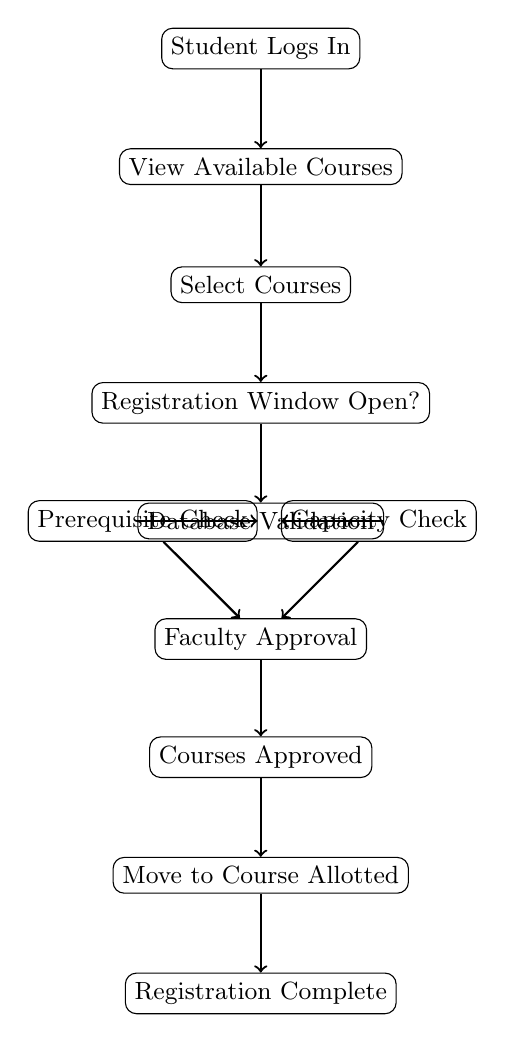
\begin{tikzpicture}[
  font=\small,
  node distance=1.5cm,
  every node/.style={rectangle, draw, rounded corners},
  arrow/.style={->, thick}
]

% Define nodes
\node (start) {Student Logs In};
\node (view) [below of=start] {View Available Courses};
\node (select) [below of=view] {Select Courses};
\node (regcheck) [below of=select] {Registration Window Open?};
\node (validcheck) [below of=regcheck] {Database Validation};
\node (prereq) [left of=validcheck] {Prerequisite Check};
\node (capacity) [right of=validcheck] {Capacity Check};
\node (facultyapp) [below of=validcheck] {Faculty Approval};
\node (approved) [below of=facultyapp] {Courses Approved};
\node (courseallot) [below of=approved] {Move to Course Allotted};
\node (complete) [below of=courseallot] {Registration Complete};

% Draw connections
\draw [arrow] (start) -- (view);
\draw [arrow] (view) -- (select);
\draw [arrow] (select) -- (regcheck);
\draw [arrow] (regcheck) -- (validcheck);
\draw [arrow] (validcheck) -- (prereq);
\draw [arrow] (validcheck) -- (capacity);
\draw [arrow] (prereq) -- (facultyapp);
\draw [arrow] (capacity) -- (facultyapp);
\draw [arrow] (facultyapp) -- (approved);
\draw [arrow] (approved) -- (courseallot);
\draw [arrow] (courseallot) -- (complete);

\end{tikzpicture}
\end{center}

\subsection{Fee Payment Workflow}

\begin{center}
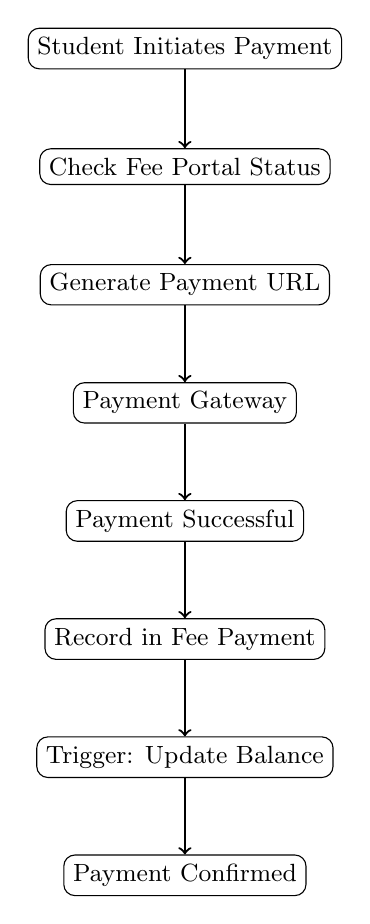
\begin{tikzpicture}[
  font=\small,
  node distance=1.5cm,
  every node/.style={rectangle, draw, rounded corners},
  arrow/.style={->, thick}
]

\node (start) {Student Initiates Payment};
\node (check) [below of=start] {Check Fee Portal Status};
\node (initiate) [below of=check] {Generate Payment URL};
\node (gateway) [below of=initiate] {Payment Gateway};
\node (success) [below of=gateway] {Payment Successful};
\node (record) [below of=success] {Record in Fee Payment};
\node (trigger) [below of=record] {Trigger: Update Balance};
\node (confirm) [below of=trigger] {Payment Confirmed};

\draw [arrow] (start) -- (check);
\draw [arrow] (check) -- (initiate);
\draw [arrow] (initiate) -- (gateway);
\draw [arrow] (gateway) -- (success);
\draw [arrow] (success) -- (record);
\draw [arrow] (record) -- (trigger);
\draw [arrow] (trigger) -- (confirm);

\end{tikzpicture}
\end{center}

\subsection{Leave Management Workflow}

\begin{center}
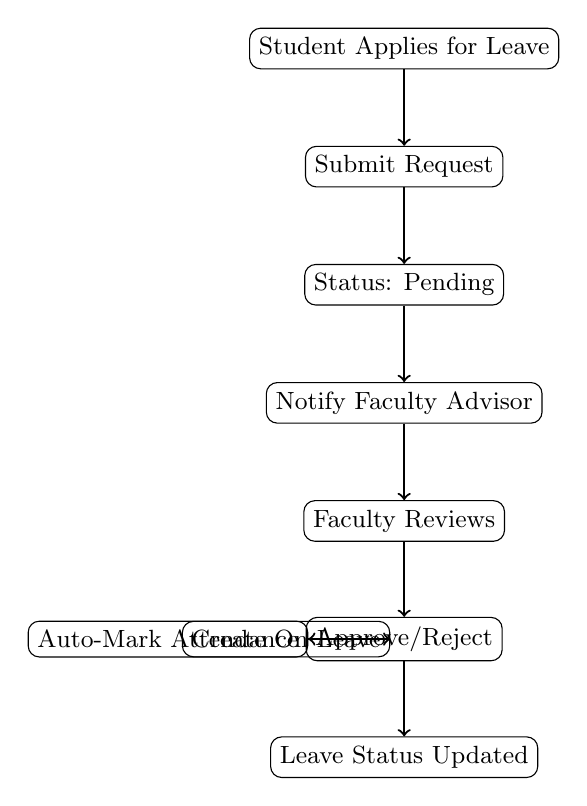
\begin{tikzpicture}[
  font=\small,
  node distance=1.5cm,
  every node/.style={rectangle, draw, rounded corners},
  arrow/.style={->, thick}
]

\node (apply) {Student Applies for Leave};
\node (submit) [below of=apply] {Submit Request};
\node (pending) [below of=submit] {Status: Pending};
\node (notify) [below of=pending] {Notify Faculty Advisor};
\node (review) [below of=notify] {Faculty Reviews};
\node (decision) [below of=review] {Approve/Reject};
\node (createleave) [left of=decision] {Create On Leave};
\node (markatt) [left of=createleave] {Auto-Mark Attendance};
\node (complete) [below of=decision] {Leave Status Updated};

\draw [arrow] (apply) -- (submit);
\draw [arrow] (submit) -- (pending);
\draw [arrow] (pending) -- (notify);
\draw [arrow] (notify) -- (review);
\draw [arrow] (review) -- (decision);
\draw [arrow] (decision) -- (createleave);
\draw [arrow] (createleave) -- (markatt);
\draw [arrow] (decision) -- (complete);

\end{tikzpicture}
\end{center}

\newpage

\section{Data Integrity and Constraints}

\subsection{Primary Key Constraints}

All tables implement primary key constraints on unique identifier columns. Composite keys are used where multiple columns uniquely identify a record (e.g., Course\_Registration uses student\_id, course\_offering\_id, and semester).

\subsection{Foreign Key Constraints}

Foreign keys enforce referential integrity across tables. Key relationships include:
\begin{itemize}
    \item Students → Users (student\_id → user\_id)
    \item Students → Departments (department\_id → dept\_id)
    \item Courses → Departments (department\_id → dept\_id)
    \item Course\_Offerings → Faculty, Courses, Discipline
    \item Grades → Students, Course\_Offerings
    \item Attendance → Students, Course\_Offerings
    \item Fee\_Payment → Students
    \item Leave\_Requests → Students
    \item ON DELETE CASCADE applied where appropriate to maintain consistency
\end{itemize}

\subsection{Check Constraints}

\begin{itemize}
    \item role IN ('Admin','Faculty','Student') - User roles
    \item credits > 0 - Course credits must be positive
    \item grade IN ('Ex','A','B','C','D','E','P','F') - Valid grade scale
    \item status IN ('Present','Absent','On\_Leave') - Attendance status
    \item leave\_status IN ('Pending','Approved','Rejected') - Leave request status
    \item amount\_paid >= 0 - Non-negative fee payments
    \item capacity > 0 - Room and course capacity constraints
    \item cgpa BETWEEN 0 AND 10 - CGPA valid range
    \item start\_time < end\_time - Time validity for class booking
    \item job\_type IN ('Intern','Placement') - CDC opportunity type
    \item selected=FALSE OR approved=TRUE - Registration logic (can't approve without selecting)
    \item config\_id = 1 - Only one system config allowed
\end{itemize}

\newpage

\section{API Endpoint Summary}

\subsection{Student APIs}

\begin{table}[H]
\centering
\small
\begin{tabular}{|p{4cm}|p{2cm}|p{5cm}|}
\hline
\textbf{Endpoint} & \textbf{Method} & \textbf{Purpose} \\
\hline
/signup & POST & User registration \\
/login & POST & Authentication \\
/student/profile/:id & GET & Profile retrieval \\
/student/profile & POST & Profile update \\
/student/registrations/:id & GET & View available courses \\
/student/registration & POST & Select/deselect courses \\
/student/courses/:id & GET & View enrolled courses \\
/student/:id/fee-status & GET & Fee information \\
/student/:id/pay & POST & Initiate payment \\
/student/payment-success & POST & Record payment \\
/student/:id/payment-history & GET & View payments \\
/student/:id/current-sgpa & GET & Current semester GPA \\
/student/:id/cgpa & GET & Overall CGPA \\
/student/:id/current-courses & GET & Current semester courses \\
/student/:id/semester/:sem/transcript & GET & Semester transcript \\
/student/:id/attendance & GET & Attendance summary \\
/student/:id/feedback-courses & GET & Eligible feedback courses \\
/student/submit-feedback & POST & Submit feedback \\
/student/:id/submitted-feedback & GET & View submitted feedback \\
/student/apply-leave & POST & Apply for leave \\
/student/:id/leave-requests & GET & View leave status \\
/student/:id/exams & GET & View exam schedule \\
/student/:id/timetable & GET & View class timetable \\
/student/:id/supplementary-exams & GET & View supplementary exams \\
/student/:id/faculty-advisor & GET & View advisor \\
\hline
\end{tabular}
\end{table}

\subsection{Faculty APIs}

\begin{table}[H]
\centering
\small
\begin{tabular}{|p{4cm}|p{2cm}|p{5cm}|}
\hline
\textbf{Endpoint} & \textbf{Method} & \textbf{Purpose} \\
\hline
/faculty/profile/:id & GET & Profile retrieval \\
/faculty/profile & POST & Profile update \\
/faculty/:id/courses & GET & All assigned courses \\
/faculty/:id/current-courses & GET & Current semester courses \\
/faculty/course/:cid/students & GET & Course student roster \\
/faculty/mark-attendance & POST & Mark attendance \\
/faculty/upload-grades & POST & Upload grades \\
/faculty/pending/:fid & GET & Pending approvals \\
/faculty/student-courses/:sid & GET & Student pending courses \\
/faculty/approve & POST & Approve registration \\
/faculty/:id/leave-requests & GET & Pending leave requests \\
/faculty/leave-action & POST & Approve/reject leave \\
/faculty/:id/advisory-students & GET & Advisees list \\
/faculty/course/:cid/feedbacks & GET & Course feedback \\
/faculty/buildings & GET & Available buildings \\
/faculty/available-slots & GET & Available rooms \\
/faculty/book-class & POST & Book extra class \\
/faculty/book-rooms & POST & Book room \\
/faculty/:id/bookings & GET & My bookings \\
/faculty/:id/schedule & GET & My class schedule \\
\hline
\end{tabular}
\end{table}

\subsection{Admin APIs}

\begin{table}[H]
\centering
\small
\begin{tabular}{|p{4cm}|p{2cm}|p{5cm}|}
\hline
\textbf{Endpoint} & \textbf{Method} & \textbf{Purpose} \\
\hline
/admin/system-config & GET & Get configuration \\
/admin/declare-results & POST & Declare examination results \\
/admin/run-query & POST & Execute SQL queries \\
/student/:id/results & GET & View student results \\
/student/:id/grades & GET & View student grade history \\
\hline
\end{tabular}
\end{table}

\newpage

\section{Banking Module}

The banking module provides complementary financial services within the ERP ecosystem.

\subsection{Banking Database Schema}

\subsubsection{Customers Table}
\begin{itemize}
    \item customer\_id (Primary Key)
    \item email (Unique constraint)
    \item password (bcrypt hashed)
    \item name, phone, created\_at
\end{itemize}

\subsubsection{Accounts Table}
\begin{itemize}
    \item customer\_id (Primary Key)
    \item account\_id (Unique constraint)
    \item balance (Non-negative check)
    \item account\_type (savings/current check constraint)
    \item status (active/inactive/closed check constraint)
    \item created\_at
\end{itemize}

\subsubsection{Transactions Table}
\begin{itemize}
    \item transaction\_id (Primary Key)
    \item account\_id (Foreign Key)
    \item transaction\_type (credit/debit check constraint)
    \item amount (Positive check constraint)
    \item created\_at
\end{itemize}

\subsubsection{Transfers Table}
\begin{itemize}
    \item transfer\_id (Primary Key)
    \item from\_account, to\_account (Foreign Keys, different accounts check)
    \item amount (Positive check)
    \item status (pending/completed/failed check)
    \item created\_at
\end{itemize}

\subsection{Banking Functionalities}

\begin{enumerate}
    \item \textbf{Sign Up / Login}: Customer registration and authentication with email uniqueness
    
    \item \textbf{Account Management}: Create savings/current account with balance tracking
    
    \item \textbf{Balance Enquiry}: Check account balance and account details
    
    \item \textbf{Deposit}: Credit funds to account via transaction
    
    \item \textbf{Withdrawal}: Debit funds from account with balance validation
    
    \item \textbf{Fund Transfer}: Transfer money between accounts with validation and status tracking
    
    \item \textbf{Transaction History}: View all transactions and transfers
    
    \item \textbf{Payment Processing}: Process payments with confirmation and receipt
\end{enumerate}

\newpage

\section{Technical Implementation Details}

\subsection{Backend Architecture}

The Express.js backend (port 5000) implements RESTful API endpoints following these patterns:

\begin{enumerate}
    \item \textbf{Request Validation:} All endpoints validate input parameters before processing
    \item \textbf{Database Connection Pooling:} Uses pg library for connection management
    \item \textbf{Error Handling:} Comprehensive error catching with specific HTTP status codes
    \item \textbf{Transaction Support:} Uses database transactions for multi-step operations
    \item \textbf{Async/Await:} All database operations use async/await pattern
    \item \textbf{CORS Support:} Cross-origin requests enabled for frontend communication
\end{enumerate}

\subsection{Frontend Architecture}

The React frontend implements:

\begin{enumerate}
    \item \textbf{Role-Based Routing:} Different dashboards for Student/Faculty/Admin roles
    \item \textbf{Local Storage:} Caches user\_id and role after login
    \item \textbf{Component Hierarchy:} Modular components for each functionality
    \item \textbf{Bootstrap Styling:} Responsive design with Bootstrap classes
    \item \textbf{State Management:} React hooks (useState, useEffect) for component state
    \item \textbf{API Integration:} axios/fetch calls to backend endpoints
\end{enumerate}

\subsection{Database Implementation}

\begin{enumerate}
    \item \textbf{Schema Normalization:} Tables designed in BCNF (Boyce-Codd Normal Form)
    \item \textbf{Constraint Enforcement:} All business rules implemented as database constraints
    \item \textbf{Trigger Automation:} 10+ triggers automate workflows and maintain consistency
    \item \textbf{View Abstraction:} 20+ views simplify complex queries
    \item \textbf{Stored Procedures:} Critical operations wrapped in procedures (make\_payment, apply\_leave, etc.)
    \item \textbf{Indexing:} Strategic indexes on frequently queried columns
\end{enumerate}

\newpage

\section{Security Considerations}

\subsection{Authentication}

\begin{itemize}
    \item Bcrypt password hashing with 10-round salt
    \item Legacy migration support for plain-text passwords (automatically upgraded)
    \item JWT-like session management via localStorage
    \item Automatic password validation (uppercase, digit, special character required)
\end{itemize}

\subsection{Authorization}

\begin{itemize}
    \item Role-based access control (Student, Faculty, Admin)
    \item API endpoints validate user role before granting access
    \item Database constraints enforce role-specific permissions
\end{itemize}

\subsection{Data Protection}

\begin{itemize}
    \item SQL injection prevention via parameterized queries
    \item Admin query console blocks dangerous DDL/DCL operations
    \item Query timeout (5 seconds) prevents resource exhaustion
    \item Result limit (100 rows max) on SELECT queries
    \item Query logging for audit trail
\end{itemize}

\subsection{Data Validation}

\begin{itemize}
    \item Check constraints on all critical columns
    \item Foreign key integrity enforcement
    \item Composite key uniqueness across tables
    \item Business logic validation in stored procedures
\end{itemize}

\newpage

\section{Performance Optimization}

\subsection{Database Optimization}

\begin{itemize}
    \item Indexes on frequently searched columns (student\_id, faculty\_id, course\_offering\_id)
    \item Query views pre-compute complex joins
    \item Stored procedures reduce network round trips
    \item Composite primary keys prevent duplicate entries
\end{itemize}

\subsection{API Optimization}

\begin{itemize}
    \item Connection pooling for database connections
    \item Async/await for non-blocking operations
    \item CORS caching headers for static responses
    \item Pagination support via LIMIT and OFFSET (if needed)
\end{itemize}

\subsection{Scheduled Cleanup}

\begin{itemize}
    \item Cron jobs delete old records (exams, feedback, leave) to maintain table size
    \item Prevents performance degradation over time
    \item Implements data retention policies
\end{itemize}

\newpage

\section{Deployment and Maintenance}

\subsection{Database Setup}

\begin{enumerate}
    \item Create PostgreSQL database
    \item Execute schema files in order (01\_users.sql through 31...)
    \item Run constraints.sql to add validation constraints
    \item Execute triggers.sql to set up automation
    \item Load test data via test\_data\_inserts.sql
\end{enumerate}

\subsection{Backend Deployment}

\begin{enumerate}
    \item Install Node.js and npm dependencies: \texttt{npm install}
    \item Configure database connection in db.js
    \item Start backend: \texttt{node app.js}
    \item Backend runs on port 5000
\end{enumerate}

\subsection{Frontend Deployment}

\begin{enumerate}
    \item Install React dependencies: \texttt{npm install}
    \item Update API base URL in services/api.js
    \item Start development server: \texttt{npm start}
    \item Build for production: \texttt{npm run build}
\end{enumerate}

\newpage

\section{Conclusion}

The ERP Clone project successfully demonstrates a comprehensive enterprise resource planning system tailored for educational institutions. By combining academic management (EIMS) with banking services within a single platform, the system showcases how modern web technologies can be leveraged to streamline institutional operations.

The system emphasizes:

\begin{itemize}
    \item \textbf{Modularity:} Clean separation between frontend, backend, and database layers
    \item \textbf{Data Integrity:} Comprehensive constraints and triggers ensure consistency
    \item \textbf{Workflow Automation:} Database-driven automation reduces manual errors
    \item \textbf{Role-Based Access:} Distinct functionality for students, faculty, and administrators
    \item \textbf{Scalability:} Normalized schema design supports future expansion
    \item \textbf{Security:} Multiple layers of authentication, authorization, and validation
\end{itemize}

Future enhancements could include:
\begin{itemize}
    \item Mobile app versions (React Native)
    \item Real payment gateway integration
    \item Advanced analytics and reporting dashboards
    \item Communication module (notifications, messaging)
    \item Document management system
    \item AI-based course recommendations
\end{itemize}

\end{document}